\section{Background and Objectives}\label{sec:background}

The objective is to have our humanoid Jaemi Hubo throw a regulation Major League Baseball ball from the pitchers mound across home plate, a distance of 60.5 feet (18.4 m).  
The regulation Major League Baseball ball has a circumference between $9 - 9\frac{1}{4}$ inches (229-235 mm) and weights $5-5\frac{1}{4}$ ounces (142-149 g)\cite{mlbrules}.  
When children are asked to throw the first pitch it is typical for them to stand halfway between the pitchers mound and home plate.
The robot used to throw the pitch, Jaemi Hubo, stands 130 cm tall, the average height of a ten year old child.
To properly fit the stature of the robot the pitch will be given from half the regulation distance.
Using the well known projectile motion formulation it is determined that the robot must have an end effector velocity of 9.47 $\frac{m}{s}$ at $45^o$ when it releases the ball in order for it to cross the plate.
%When Hubo moved to and from the field Jaemi would 

Along with the technical challenges the primary objective sought to anthropomorphize robotic pitching.  
As such Jaemi Hubo was outfitted with a uniform shirt and cap.
In addition Jaemi gestures the crowd by waving its hand when entering and exiting the field.
Thus, beyond simply pitching, the challenge was to engage the audience hence the \textit{Science Night at the Ballpark}.


%is the highly articulated 40 degree of freedom (DOF) adult-size humanoid 


%The pitch is in front of an audience of over 30,000 with thousands more watching on television.
%Failure to successfully throw the ball is not an option.
%Learning from past attempts of dexterous robots under throwing the ball 

Completing the technical objective with a humanoid consists of two major parts: 1) end-effector velocity control and 2) balance/stabilization. 
There are many examples of throwing/pitching machines made by commercial companies such as Louisville Slugger$^{TM}$, Jugs$^{TM}$, and Atec$^{TM}$ to name a few.  
These devices typically contain one to two fly wheels that the ball travels through in order to be launched or a spring loaded arm that is compressed and released.
None of these robots are humanoid or bipedal.
All of these devices are well planted to the ground to ensure stability.

Robots designed for throwing come in many shapes and sizes depending on the objective.  
2-DOF mechanisms are able to throw in $R^3$ space with the correct kinematic structure.  
Visual feedback was used in the basketball throwing robot ($\leq 7$ DOF) by Hu et al.~\cite{5649335} achieving an accuracy of 99\% at distances $\leq$ 3 m.  
This robot was fixed to the ground to guarantee stability.
The PhillieBot\footnote{PhillieBot Video: http://youtu.be/ShId-vZ-ZEY} made by the GRASP Lab at the University of Pennsylvania was the robot that threw the first pitch at the first annual Philadelphia Science Festival \textit{Science Night at the Ballpark} in 2011.  
The PhillieBot consisted of a $\leq 7$ DOF arm with a pneumatic wrist actuator to increase end-effector velocity at the release point.  
The arm was attached to a wheeled mobile platform.
None of the latter robots are anthropomorphic thus they limit the audience engagement.

Kim et al. \cite{5686315,JooH2011438} takes the research to the next level with finding optimal overhand and sidearm throwing motions for a high degree of freedom humanoid computer model.  
The model consists of 55-DOF and is not fixed to mechanical ground or a massive base.  
Motor torques are then calculated to create both sidearm and overhand throws that continuously satisfies the zero-moment-point stability criteria~\cite{4309277}.  

\begin{figure}[t]
  \centering
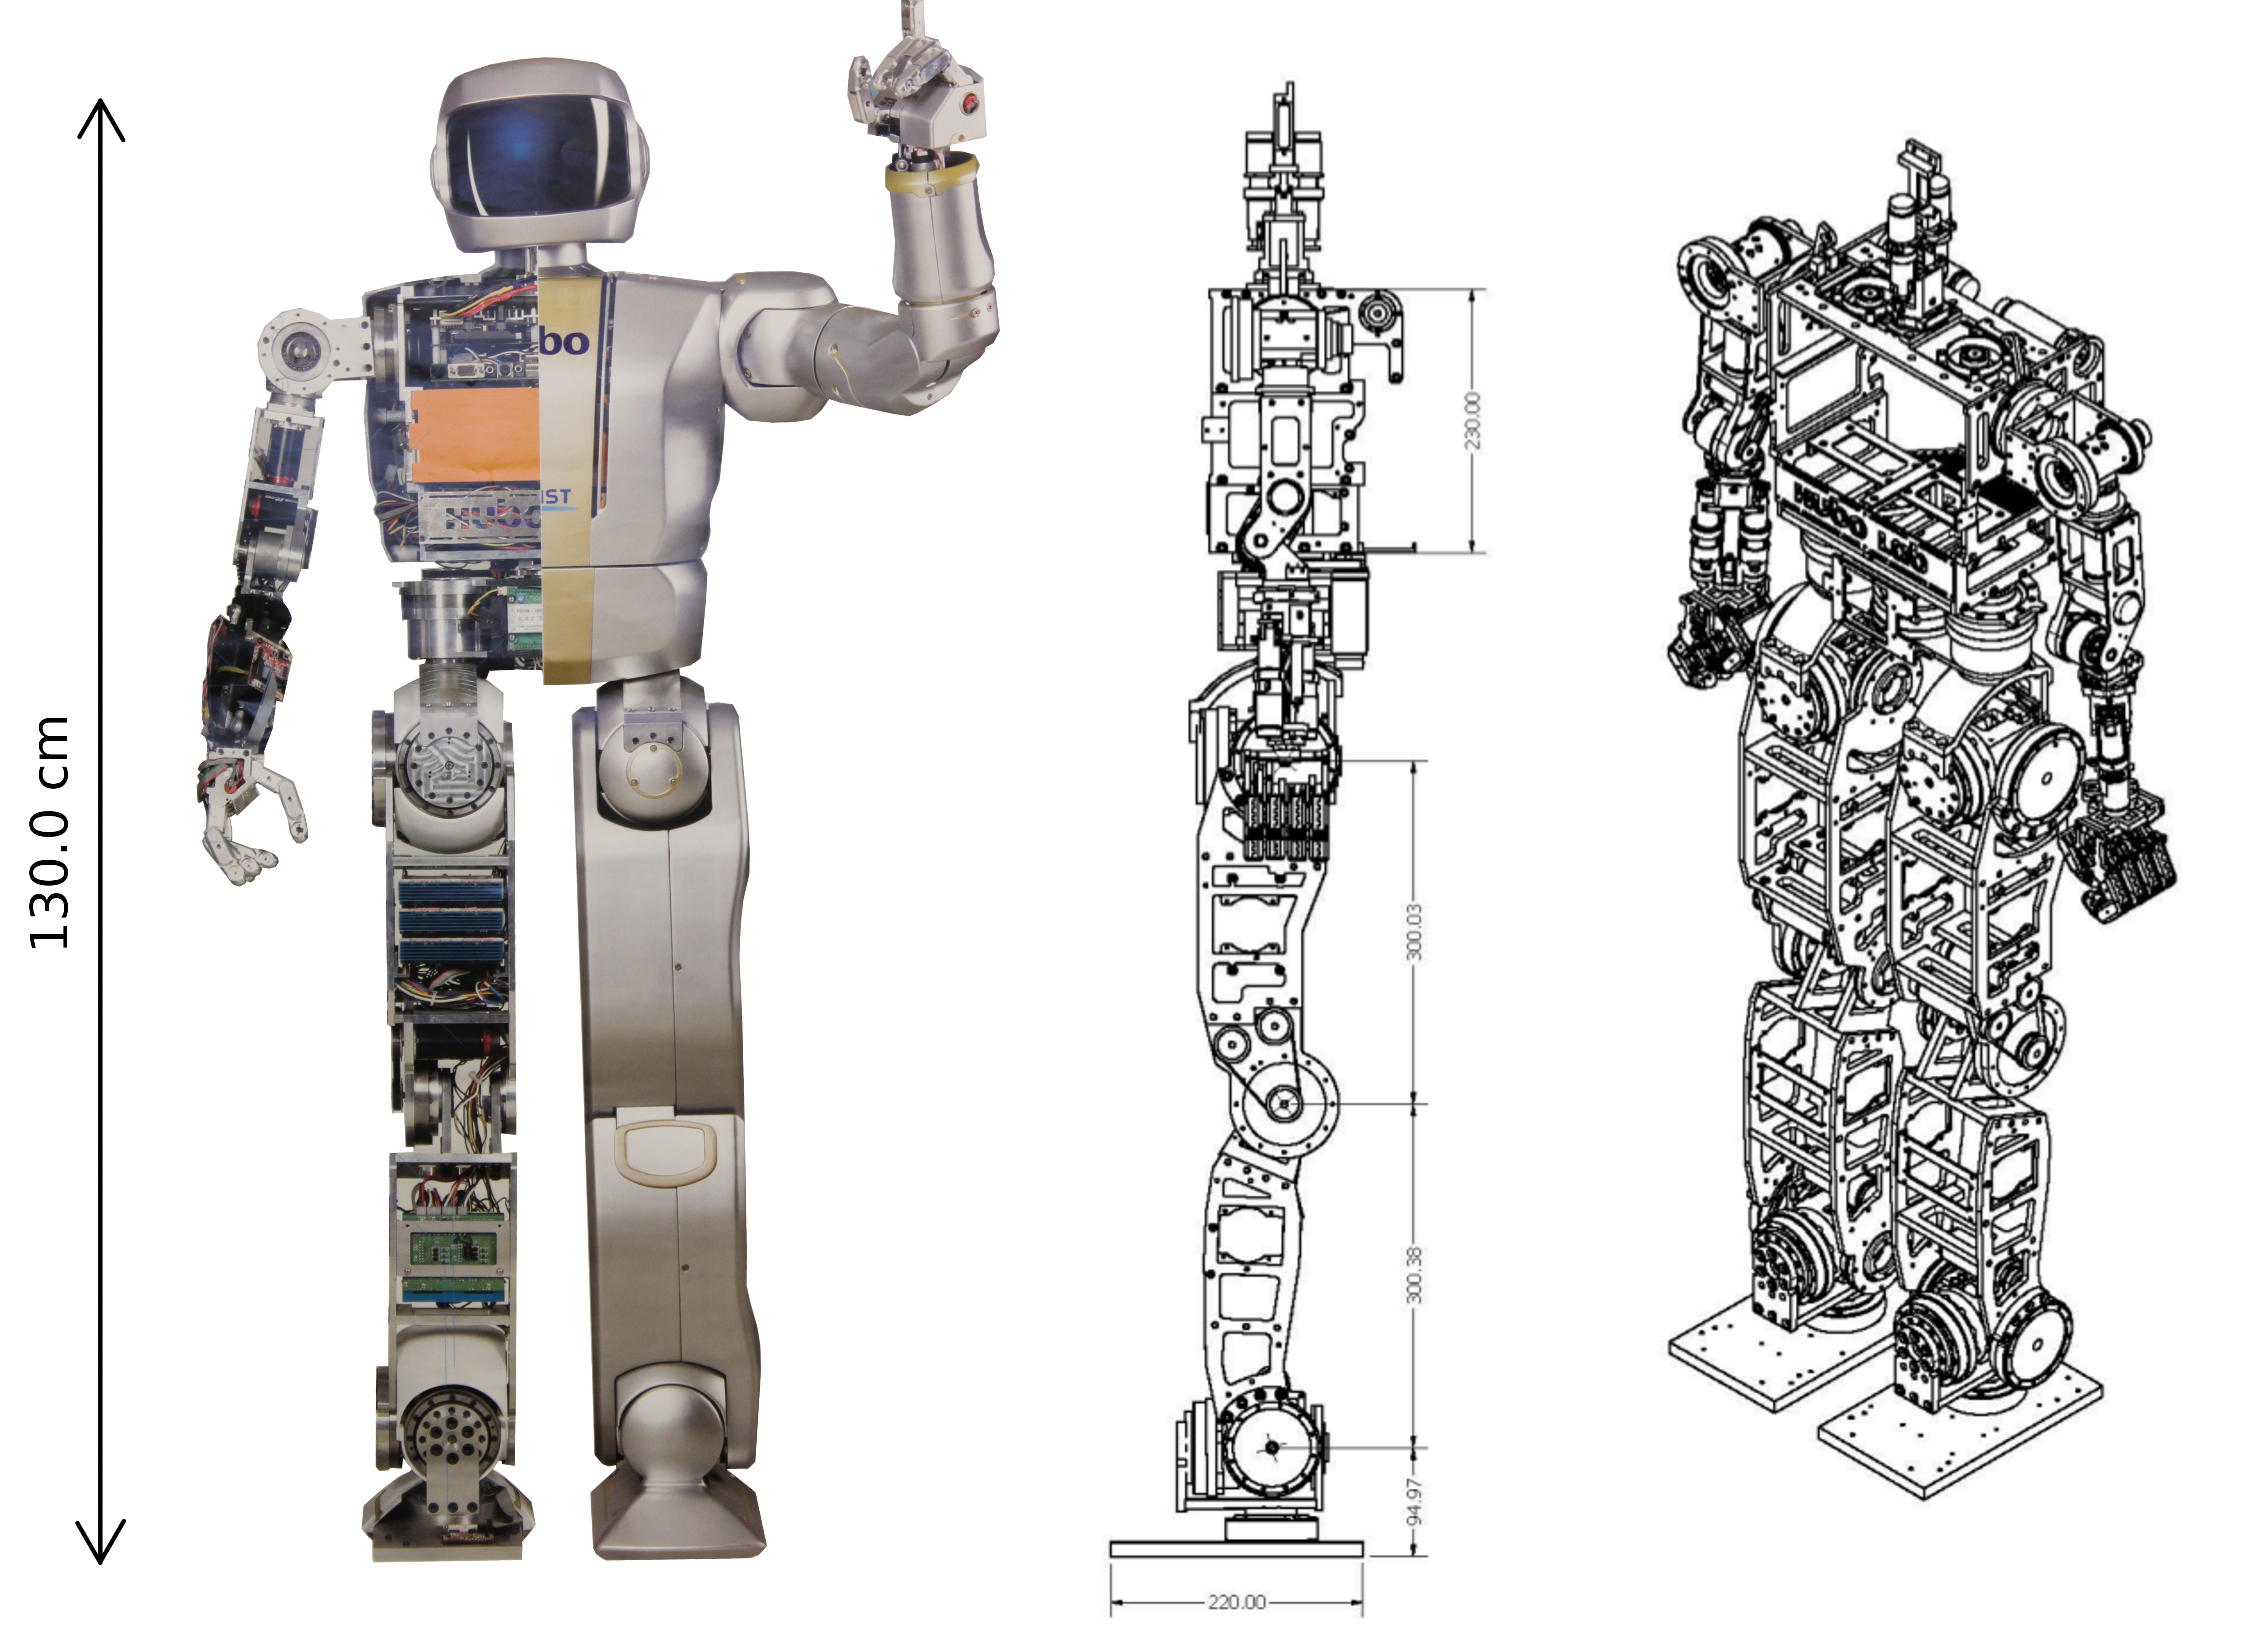
\includegraphics[width=1.0\columnwidth]{./pix/huboExample.png}
  \caption{Jaemi Hubo is a 130 cm tall 37 kg 40-DOF highly articulated, high-gain position controlled, full-size humanoid.}
  \label{fig:huboFig}
\end{figure}


%% needs to be modified
The highly articulated 40-DOF full-size humanoid Jaemi Hubo (Fig.~\ref{fig:huboFig}) is the platform focused on in this work.  Jaemi Hubo is a high-gain, position-controlled biped humanoid weighing 37 kg and standing 130 cm tall.  It is designed and made by Dr. Jun-Ho Oh director of the Hubo Lab at the Korean Advanced Institute of Science and Technology (KAIST).  Jaemi has been located at the Drexel Autonomous Systems Lab (DASL) at Drexel University since the Fall of 2008.  DASL has extensive experience with the Jaemi Hubo KHR-4 platform in key areas needed to complete this work.  Balancing was explored when developing a real-time zero moment point (ZMP) preview control system for stable walking~\cite{5686276}.  A full-scale safe testing environment designed for experiments with Jaemi Hubo was created using DASL's Systems Integrated Sensor Test Rig (SISTR)~\cite{5686325}.  Additionally all algorithms are able to be tested on miniature and virtual versions of Jaemi Hubo prior to testing on the full-size humanoid through the creation of a surrogate testing platform for humanoids~\cite{5379582}.



%Such a mechanism can choose its release point or its end-effector velocity but not both.  
%Mechanisms containing 3 or more DOF with the correct kinematic structure are able to throw in $R^3$ and choose both the release point and the end-effector velocity simultaneously.

% need to modify
%Low degree of freedom throwing machines/robots are common.  Typical throwing robots have between one and three degrees of freedom (DOF)~\cite{509405, Lynch97dynamicnonprehensile, 5152525, 509335, springerlink:10.1007/s10015-006-0401-0}.  All of these mechanisms are limited to throwing in a plane.   Sentoo et al.~\cite{4651142} achieved an end-effector velocity of 6.0 m/s and can throw in $R^3$ space using it's Barret Technology Inc 4-DOF arm with a $360^o$ rotation base yaw actuator.  These low degree of freedom throwing robots are either physically attached/planted to the mechanical ground or have a base that is significantly more massive then the arm. 

%Haddadin et al.\cite{6094757} used their 7-DOF arm and a 6-DOF force torque sensor with standard feedback methods to dribble a basket ball.  In addition Zhikun et al.~\cite{6094892} used reinforcement learning to teach their 7-DOF planted robot arm to play ping-pong.  Likewise Schaal et al.~\cite{schaal01/BIRG} taught their high degree of freedom (30-DOF) humanoid robot to hit a tennis ball using on-line special statistical learning methods. 